\section{Experiments and Compiled Verification Costs}
\label{sec:experiments}

Three complementary studies test the protocol. Deterministic adversarial vectors test acceptance and rejection. Exact enumeration and seeded Monte Carlo test committee and selection mechanisms. A compiled verifier runs on a real private Algorand ledger to measure cryptographic checking costs. These are different kinds of evidence and are reported separately.

Each study preserves its design, configuration, input vectors or raw observations, source hashes, and output hashes. Development preceded the locally frozen final designs; this is not external preregistration. Later integration and repair checks are labeled as such. Designed attacks establish concrete conformance results, not estimated real-world attack frequencies.

\subsection{Commitment, semantics, and publication}

An independent JavaScript implementation checks canonical bytes and tree openings against the Python reference. The suite covers 23 canonical vectors, every tree count from 1 through 64, and every valid index: 2,080 accepted openings. Another 576 invalid proof vectors exercise wrong context/count/index, payload changes, proof shape, and malformed inputs. All 2,656 decisions and the corresponding roots agree across implementations. This cross-check covers encoding and commitments; it does not describe the JavaScript tool as an independently implemented blueprint interpreter.

The semantic suite executes six valid traces across the 4-, 16-, and 64-slot profiles and both Boolean outcomes. Fifteen attacks preserve the declared leaf count and recompute valid new roots: Merkle authentication alone therefore accepts every supplied opening. The complete semantic checker rejects the fabricated traces. This intervention isolates the role of the semantic rules instead of taking credit for detecting a stale hash after an obvious edit.

Source tests distinguish unauthenticated host forgery, signature failure, scope/freshness failure, and an authentic false source. One malicious plaintext proxy can fake every apparent unsigned endpoint. The same altered objects fail pinned-source authentication. An authentic common error remains accepted as authentic input; cryptography does not turn the report into truth.

Publication tests exercise complete and missing reveals, duplicate positions, deadline boundaries, malformed challenge evidence, semantic challenges, and the intentionally accepted unchallenged fabricated trace. The source-preimage gate additionally rejects a fresh-root substitution that omits the committed snapshot. Every accepted finalization preserves complete disclosure and a full checking window; neither result asserts that an independent checker was actually online.

Five separately designed follow-up integration cases join signed-source verification, semantic replay, per-run receipts, common-result certificates, and mandatory publication. Three honest runners produce distinct trace roots and one result digest. Forged sources, unauthorized measurements, and missing traces block acceptance; an authentic common-source error remains accepted. A later independent boundary audit checks 35 valid traces and 672 memberships across both branches, irregular tree sizes, and extreme accepted integers, with no false local-fault convictions. These are retained follow-up checks, not additions retroactively called part of the primary design.

\begin{table}[t]
\centering\small
\caption{Authenticated disclosure in the real reference traces, in bytes. Common stored context/root/count and ordinary transaction framing are excluded from both sides. Two-record openings use separate paths, not a multiproof.}
\label{tab:bytes}
\begin{tabular}{rrrrr}
\toprule
Slots & Whole trace & One record & Two linked records & All record bytes\\
\midrule
4 & 2,166 & 170 & 1,433 & 1,504\\
16 & 3,356 & 234 & 468 & 2,682\\
64 & 8,156 & 299 & 598 & 7,434\\
\bottomrule
\end{tabular}
\end{table}

Table~\ref{tab:bytes} compares complete account authentication with a selected interior/decision record, and with a child plus its declared parent for a local semantic challenge. The four-slot case must include the 1,191-byte source record as its parent; this makes its two-record saving smaller. At 64 slots, the two-record evidence is 598 bytes versus an 8,156-byte whole trace, a 92.67\% reduction for that challenge. Other faults can require different records or the full semantic projection.

Local timing uses seven warmed batches per operation and retains every batch measurement. Whole-trace hashing is faster than Merkle construction at these sizes. Parsing, full semantic replay including source authentication, tree construction, and opening verification are measured separately. The result supports compact authenticated disclosure, not universal CPU acceleration. Wall-clock microbenchmarks describe this machine and implementation, not network latency or a hardware-enclave performance claim.

\subsection{Quorum conditions and output selection}

The exact quorum study covers 240 $(n,k,f)$ configurations for $1\leq n\leq8$ and 3,586 fault sets. It checks the authenticity, quorum-intersection, and withholding conditions against explicit signer subsets. The 3-of-5, one-fault conflicting-certificate witness is retained as an accepted counterexample to the weaker rule. Four dependency-cover examples give minimum costs 10, 1, 20, and 1 in declared scenario units: an unconstrained vendor attack, that policy with a shared-registrar attack, a vendor-constrained policy, and the constrained policy with the shared registrar. Domain constraints improve only the dependencies they actually constrain.

The selection experiment saves 320,000 paired observations. It tests favorable probabilities $0.01$, $0.1$, $0.3$, and $0.5$; attempt counts 1, 3, 10, and 30; twenty seeds; and 1,000 episodes per cell/seed. Each raw row preserves its complete candidate outcome bitmask, so first-slot, best-of-$m$, and fixed-set rules use the same draws. Exact model probabilities are the primary result; pointwise Wilson intervals describe Monte Carlo agreement with those probabilities, not field uncertainty.

At $p=0.1,m=30$, best-of-$m$ succeeds in 95.63\% of episodes, compared with the exact 95.7609\%. The prescribed first slot is favorable in 9.97\%. Suppressing every unfavorable first-slot result makes 100\% of the finalized results favorable while completing only 9.97\% of authorizations. The experiment reproduces both the manipulation and the missing-result signal that reveals it.

\begin{figure}[!htbp]
\centering
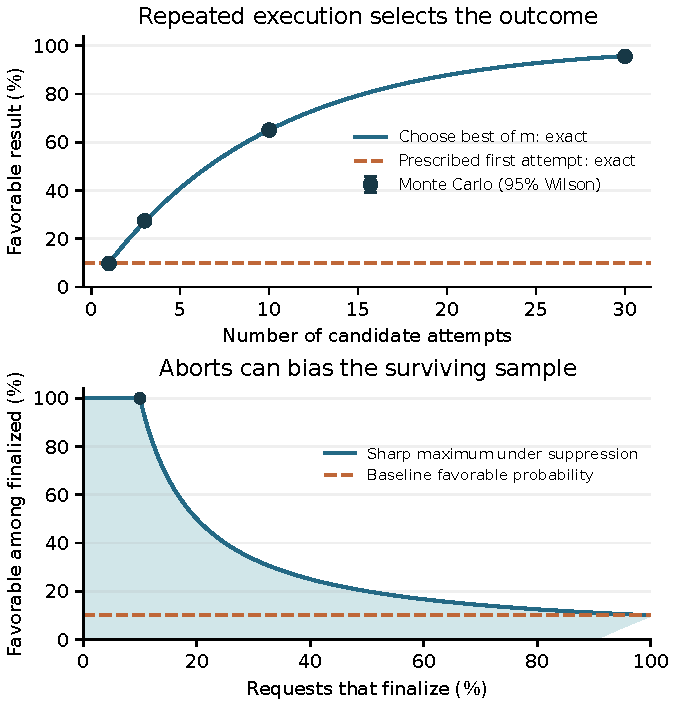
\includegraphics[width=\linewidth]{figures/selection-integrity.pdf}
\caption{Selection integrity at baseline favorable probability 0.1. Top: exact retry advantage and Monte Carlo estimates; intervals are pointwise 95\% Wilson intervals. Bottom: the sharp interval obtainable by outcome-dependent suppression at each completion rate. The upper boundary reaches 100\% when only favorable requests complete. The shaded region is an analytic bound, not an empirical confidence interval.}
\label{fig:selection}
\end{figure}

An exhaustive eight-element probability-space check evaluates 65,280 event/selection pairs with no violation of either sharp conditional bound. A separate deterministic toy computation repeats 10,000 fixed requests thirty times each: all 300,000 re-executions preserve their initial result. This checks the restart construction; it is not evidence that a hosted LLM API or GPU kernel is deterministic. Certificate and attempt tests also preserve the accepted hidden-restart counterexample for a slot policy that does not fix execution randomness.

\subsection{Measured AVM costs}
\label{sec:avm}

The cryptographic kernel is compiled with PuyaPy 5.7.1, optimization level 2, targeting AVM 11, and executed on native go-algorand 5.0.3 (commit \texttt{2dc9524e}) with private consensus v42. It checks stored context and count, fixed-width indices, proof length, payload and leaf hashes, every sibling, the root wrapper, and optionally an Ed25519 signature on the stored result/trace projection. The approval program is 624 bytes; the clear program is 2 bytes. The measured profile uses power-of-two counts; padded trees are covered by the independent off-chain conformance study.

\begin{table}[t]
\centering\small
\caption{Complete cryptographic verification kernel, all indices. Group costs include required 29-unit budget calls; each reported group also includes one zero-value self-payment. Fees are base fees before argument-size surcharges.}
\label{tab:avm}
\begin{tabular}{llrrr}
\toprule
Slots & Method & Main call & Worst group & App calls / fee (ALGO)\\
\midrule
4 & Membership & 384--386 & 386 & 1 / 0.002\\
16 & Membership & 540--544 & 544 & 1 / 0.002\\
64 & Membership & 696--702 & 731 & 2 / 0.003\\
4 & Signed & 2,345--2,347 & 2,434 & 4 / 0.005\\
16 & Signed & 2,501--2,505 & 2,592 & 4 / 0.005\\
64 & Signed & 2,657--2,663 & 2,750 & 4 / 0.005\\
\bottomrule
\end{tabular}
\end{table}

The study checks all 84 positions across the three sizes for both methods, giving 168 index/method measurements. Another 24 accepted groups vary payload sizes from 256 to 4,096 bytes; 18 use actual reference trace records. Those 42 groups were submitted and confirmed, without extra-budget simulation overrides. Forty-five negative controls test malformed proofs, state/context mismatch, signatures, and actual resource limits. A fresh-ledger reproduction agrees on opcode costs and acceptance behavior; transaction identities, rounds, and RPC timings need not match.

The precise result matters. A 64-leaf leftmost path costs 702 units and needs a second application call; quoting only the 696-unit rightmost path would hide that boundary. An application call contributes 700 units to the pool, while a payment contributes none. A verifier grouped with fifteen payments still lacks the signature budget. The signed path includes a 1,900-unit \texttt{ed25519verify\_bare} and its additional message hash \cite{algorandopcodes2026,algorandcosts2026}.

For this tree encoding, the membership hash-only lower bound is
\[
35\bigl(\lceil\log_2 n\rceil+3\bigr),
\]
including payload hashing, the leaf envelope, and root wrapper. It is 175, 245, and 315 units at 4, 16, and 64 leaves. Table~\ref{tab:avm} includes the parsing of binary arguments, bounds, loop, state, and comparison work omitted by that lower bound. It still does not include blueprint semantic replay, registration, TEE document verification, or the full reveal/settlement state machine.

The whole-trace single-buffer hash baseline costs 71 units for the 2,166- and 3,356-byte traces. The 8,156-byte trace exceeds the individual 4,096-byte argument/stack limit; a streaming whole-trace baseline is feasible in principle but is not measured here. Consensus v42 permits larger combined arguments with a fee surcharge of 0.1 microAlgo per byte above 2,048, rounded up at the group level, while retaining the individual-value limit \cite{algorandfees2026}. Thus a 4,096-byte leaf succeeds with a surcharge, whereas a payload plus proof can exceed the free argument allowance even when the payload alone fits. Fees buy argument capacity, not opcode budget.

The test application's setup reserves 378,500 microAlgo of minimum balance for one integer and five byte-valued global slots plus the application base. That is neither a per-proof fee nor an estimate of a complete market's storage requirement. The private-ledger measurements establish practical compact verification under pinned rules. Public-chain latency, production publication storage, and complete-market costs remain measurements for the deployment study.
